\documentclass[12pt]{iopart}
%\documentclass[prl,nofootinbib,twocolumn,floatfix,showpacs]{revtex4}
%Uncomment next line if AMS fonts required
%\usepackage{iopams}  

\usepackage{graphicx}
\usepackage{amsmath}
\usepackage{amssymb}
\setlength{\topmargin}{0in}

\begin{document}
\title{Anharmonicity, mode-coupling and entropy in a fluctuating
  native protein}

\author{A. Kabak{\c c}{\i}o{\u g}lu$^\dagger$, D. Y{\" u}ret$^*$, M. G{\" u}r$^*$, B. Erman$^{*,\dagger}$}
\address{Colleges of Sciences$^\dagger$ and Engineering$^*$, Ko{\c c} University, Sar{\i}yer, 34450, {\. I}stanbul, Turkey}
\ead{akabakcioglu@ku.edu.tr}

%\date{\today }

\begin{abstract}
We develop a general framework for the analysis of residue
fluctuations that simultaneously incorporates anharmonicity and
mode-coupling in a unified formalism. We show that both deviations
from the Gaussian model are important for modeling the
multidimensional energy landscape of the protein Crambin (1EJG) in the
vicinity of its native state.  The effect of anharmonicity and
mode-coupling on the fluctuational entropy is on the order of a few
percent.

\end{abstract}

\pacs{87.14.E-, 87.15.-V, 87.85.J-}

% Keywords required only for MST, PB, PMB, PM, JOA, JOB? 
\vspace{2pc}
\noindent{\it Keywords}: protein dynamics, anharmonicity, mode coupling
% Uncomment for Submitted to journal title message
%\submitto{\PB}
% Comment out if separate title page not required
\maketitle

Residue fluctuations of a protein around its native state reveal
information that bridges the molecule's structural and functional
properties.  At the lowest order, these fluctuations can be treated as
a collection of independent harmonic modes, yielding ``Elastic Network
Models''~\cite{bahar1997direct,atilgan2001anisotropy}. On the other
hand, it is known that the slowest oscillatory modes of a protein are
strongly
anharmonic~\cite{hayward1994harmonic,pontiggia2007anharmonicity,yogurtcu2009statistical},
in contrast with the assumption underlying ENMs. The coupling between
different modes is another aspect of protein dynamics that is believed
to be relevant for the information/energy transfer between different
parts of the molecule~\cite{moritsugu2000vibrational,leitner2008energy} and not
captured by the harmonicity assumption.


Sampling the time evolution of a protein by using molecular dynamics
reveals a multivariate probability distribution function (pdf) $f({\bf\Delta
R})$ for the deviations of atoms (assume there are $N$ of them) from
equilibrium coordinates, i.e. $\Delta R_i = R_i - R_i^{eq}$,
$i=1,\dots,3N$. We here adopt a coarse-grained representation of this
pdf where only $C^\alpha$ atoms are considered, so that $N$ is also the
number of residues. Accordingly, $R_i^{eq}$ are the mean $C^\alpha$
coordinates corresponding to the average configuration of the protein during
the part of the trajectory that is used for the calculations. Since
the deviations from this free energy minimum should be harmonic for
sufficiently small amplitudes, Hermite polynomials - which are
orthogonal {\it wrt} a Gaussian weight function - constitute a natural
basis for representing $f({\bf\Delta R})$. First, following
Ref.~\cite{garcia1992large,yogurtcu2009statistical}, we perform the
transformation
\begin{eqnarray}
\label{eq:rotation}
{\bf \Delta r} &=& \langle {\bf\Delta R \Delta R}^T\rangle ^{-1/2} {\bf
  \Delta R}\ .
\end{eqnarray}
This diagonalizes the covariance matrix $ \Gamma\equiv\langle
{\bf\Delta R \Delta R}^T\rangle$ ($\langle \cdot\rangle$
represents averaging over the trajectory) and would give the normal
modes of the protein if fluctuations were harmonic. Otherwise, the
distribution function for $\{\Delta r_i\}$ in its most general form, can
be expressed as~\cite{flory1974moments}
\begin{small}
\begin{equation}
\label{hermite_expansion}
f({\bf\Delta r}) = \frac{1}{\sqrt{(2\pi)^{3N}}} e^{
    -\frac{1}{2}\sum_{i=1}^{3N} \Delta r_i^2} \bigg[ 1 +  \sum_{\nu=3}^\infty
 {\bf C_\nu}\cdot {\bf H}_\nu({\bf \Delta r}) \bigg]
\end{equation}
\end{small}

\noindent where ${\bf C}_\nu$ (constant) and ${\bf H}_\nu$ (derived
below) are tensors of rank $\nu$, and the dot product refers to
$\sum_{ij..k}\,C_\nu^{ij..k}\,H_\nu^{ij..k}$.  The fluctuations
$\{\Delta r_i\}$ in this mode space spanned by the eigenvectors of
$\Gamma$ are meanless, i.e., $\langle {\Delta r_i}\rangle = 0$, and
decoupled at the lowest (second) order, i.e.,
\begin{equation}
\langle {
\label{eqn:pair_corr}
  \Delta r_i^T \Delta r_j}\rangle = \delta_{ij}\ .
\end{equation}
A purely harmonic model is given by ${\bf C}_\nu = 0,\ \forall
\nu$. Note that, the atomic fluctuations
corresponding to a given mode can easily be calculated by setting to
zero all the eigenvalues except the one of interest, followed by a
back transformation of Eq.~(\ref{eq:rotation}).


Tensor Hermite polynomials can be
obtained by successive differentiation using Rodrigues' formula:
\begin{eqnarray}
\label{Rodrigues}
H_{\nu}^{ij..k}({\bf \Delta r}) &=& \frac{(-1)^\nu}{g({\bf
    \Delta r})}\,{\bf\nabla}^{ij..k}\,g({\bf \Delta r})\ .
\end{eqnarray}
Above, $g({\bf x}) = (2\pi)^{3N/2}\exp(-{\bf x}^2/2)$ is the
multidimen{\-}sional Gaussian distribution and ${\bf \nabla}^{ij..k} =
\nabla^i\nabla^j\,..\,\nabla^k$ is the gradient tensor with
$\nabla^i \equiv \partial/\partial x_i$.
The tensor coefficients that appear in $f({\bf \Delta r})$
follow from the orthogonality relation as
\begin{eqnarray} 
\label{coefs}
{\bf C}_\nu &=& \frac{1}{\nu!}\int_{-\infty}^{\infty} {\bf H}_\nu({\bf x})
f({\bf\Delta r})\, {\bf d\Delta r} =  \langle {\bf H}_\nu({\bf\Delta r})\rangle/\nu!
\label{eqn:orthogonality}
\end{eqnarray}
Therefore, the problem reduces to obtaining the expectation values of
the polynomial tensor elements for the system. At the lowest
nonvanishing order they read
\begin{eqnarray}
\label{H3}
{\bf H}_3^{111}({\bf x}) &=& x_1^3 -3x_1 \nonumber \\
{\bf H}_3^{112}({\bf x}) &=& x_1^2x_2 -x_2 = {\bf H}_3^{121}({\bf x}) = {\bf
  H}_3^{211}({\bf x}) \nonumber \\
{\bf H}_3^{123}({\bf x}) &=& x_1x_2x_3 = {\bf H}_3^{213}({\bf x}) = \cdots
\end{eqnarray}
Higher order tensor elements can be calculated using a diagrammatic technique.
%% \begin{eqnarray}
%% \label{H4}
%% {\bf H}_4^{1111}({\bf x}) &=& x_1^4 -6x_1^2 + 3 \nonumber \\
%% {\bf H}_4^{1112}({\bf x}) &=& x_1^3x_2 - 3x_1x_2 \nonumber \\
%% &=& {\bf H}_3^{1121}({\bf x}) = {\bf H}_3^{1211}({\bf x}) = {\bf  H}_3^{2111}({\bf x}) \nonumber \\
%% {\bf H}_4^{1122}({\bf x}) &=& x_1^2x_2^2 - x_1^2 - x_2^2 + 1 \nonumber \\
%% &=& {\bf H}_4^{1212}({\bf x}) = {\bf  H}_4^{1221}({\bf x}) \nonumber \\
%% {\bf H}_4^{1123}({\bf x}) &=& x_1^2x_2x_3 - x_2x_3  \nonumber \\
%% &=& {\bf H}_4^{1231}({\bf x}) = {\bf H}_4^{1213}({\bf x}) = \cdots
%% \end{eqnarray}
A graphical representation of $H_4$ in one and two dimensions is given in Fig.\ref{Fig1}. 
\begin{figure}[h!]
  \begin{center}
    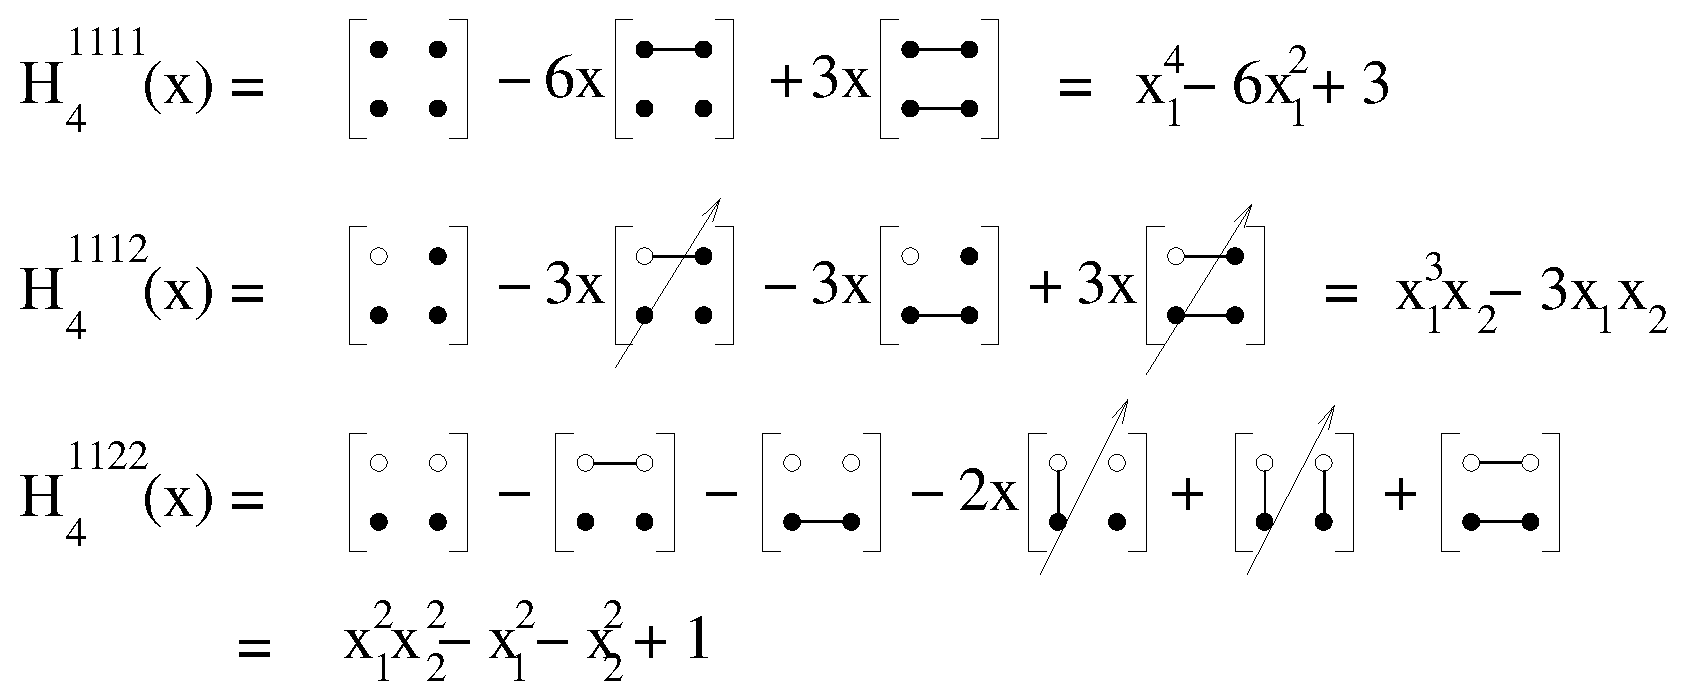
\includegraphics[width=8cm]{./fig1.eps}
  \end{center}
\caption{Graphical representation of ${\bf H}_4({\bf x})$ tensor elements in two
dimensions. Terms that vanish by virtue of Eq.~(\ref{eqn:pair_corr})
are crossed.}
\label{Fig1}
\end{figure}


The inclusion of mode-coupling necessitates consideration of mixed
indices (nondiagonal tensor elements). Here, we focus on the coupling
between mode pairs and ignore threesome and higher order mixing, i.e.,
we consider only the bi-polynomials ${\bf H}^{i_1i_2\dots
i_\nu}_\nu(\Delta r_k,\Delta r_l)$ with $i_m \in \{k,l\}$,
$k,l=1,2,\dots,3N$. At first sight, estimating the contribution of
mode-coupling even at this lowest level appears to be a formidable
task, because the number of distinct expectation values to be
extracted from the data grows combinatorially. We show below that, the
factorization property of the off-diagonal tensor elements and the
orthogonality of the modes at the second order bring a significant
reduction in complexity, which we exploit to investigate the impact of
anharmonicity and mode-coupling separately on the protein dynamics.

\subsection{Mode-coupling corrections}
The value
of a tensor element ${\bf H}^{i_1i_2\dots i_\nu}_\nu({\bf \Delta r})$
does not depend on the order of the indices due to the commutativity
of the gradient operator, $\nabla_k\nabla_l -
\nabla_l\nabla_k=0$. Therefore,
\begin{eqnarray}
{\bf H}^{i_1i_2\dots i_\nu}_\nu({\bf \Delta r}) &=& {\bf H}^p_\nu(\Delta r_k,\Delta r_l) \nonumber
\end{eqnarray}
where $p$ is the number of indices equal to $k$ (and the remaining
$\nu-p$ indices are equal to $l$). The fact that the covariance matrix
in the normal basis is diagonal further implies that
\begin{eqnarray}
\label{factorization}
{\bf H}^p_\nu({\bf \Delta r}) &=& H_p(\Delta r_1)\times H_{\nu-p}(\Delta r_2)
\end{eqnarray}
as is also evident from the Rodrigues's formula in Eq.~(\ref{Rodrigues}).

Combining Eq.~(\ref{coefs}) and Eq.~(\ref{factorization}), the Hermite
expansion in Eq.~(\ref{hermite_expansion}) can be cast into the
following form:
\begin{widetext}
\begin{eqnarray}
\label{hermite_expansion2}
f({\bf\Delta r}) &=& \frac{1}{\sqrt{(2\pi)^N}} e^{ -\sum_i \Delta
  r_i^2/2} \bigg[ 1 + \sum_i\sum_{\nu=3}^\infty
  \frac{1}{\nu!}\, \Big\langle
  H_\nu(\Delta r_i)\Big\rangle\,H_\nu(\Delta r_i) \nonumber \\
&+&  \sum_{i\ne j}\sum_{\nu=3}^\infty
  \frac{1}{\nu!}\,\sum_{p=1}^{\nu-1} {\nu\choose p} \Big\langle
  H_p(\Delta r_i)H_{\nu-p}(\Delta r_j)\Big\rangle\,H_p(\Delta r_i)H_{\nu-p}(\Delta r_j) + \sum_{i\ne j\ne k} \cdots \bigg]
\label{eqn:8}
\end{eqnarray}
\end{widetext}
The first term in Eq.~(\ref{eqn:8}) corresponds to a purely harmonic model given by
the Gaussian probability distribution
\begin{eqnarray}
\label{eqn:f0}
f_0({\bf\Delta r}) &=& \frac{1}{\sqrt{(2\pi)^N}} e^{ -\sum_i \Delta
  r_i^2/2}\ .
\end{eqnarray}
This is the starting point for most of the past studies on protein
fluctuations~\cite{cui2006normal}. The next term in Eq.~(\ref{eqn:8}) is
appreciable when the fluctuations are anharmonic, but gives no information
about mode-coupling. In fact, the most general mode-amplitude
distribution of an anharmonic model composed of decoupled modes is
\begin{eqnarray}
\label{eqn:f1}
f_1({\bf\Delta r}) &=& \frac{1}{\sqrt{(2\pi)^N}}\ e^{ -\sum_i \Delta
  r_i^2/2} \times \nonumber \\
&& \prod_i\bigg[ 1 + \sum_{\nu=3}^\infty
  \frac{1}{\nu!}\, \Big\langle
  H_\nu(\Delta r_i)\Big\rangle\,H_\nu(\Delta r_i)\bigg]
\end{eqnarray}
The approximation to the true distribution given in
Eq.~(\ref{eqn:f1}) is named $f_1$ in order to remind the reader
that it qualitatively improves on the Gaussian approximation $f_0$
of Eq.~(\ref{eqn:f0}). The difference between the full pdf given in
Eq.~(\ref{hermite_expansion2}) and the approximation $f_1$ is the
mode-coupling corrections such as
\begin{eqnarray}
\langle H_p(\Delta r_i)H_{\nu-p}(\Delta r_j)\rangle - \langle
H_p(\Delta r_i)\rangle\langle H_{\nu-p}(\Delta r_j)\rangle &\neq& 0 \nonumber
\end{eqnarray}
and higher order cumulants. Note that, marginal distributions are transparent to
such corrections
\begin{figure*}[t!]
%%   \includegraphics[width=.24\textwidth]{src/mode01.pdf}
%%   \includegraphics[width=.24\textwidth]{src/mode05.pdf}
%%   \includegraphics[width=.24\textwidth]{src/mode10.pdf}
%%   \includegraphics[width=.24\textwidth]{src/mode50.pdf}
  \includegraphics[width=.90\textwidth]{fig2.eps}
\caption{Time plots of the slowest 1$^{st}$, 5$^{th}$, 10$^{th}$, and 50$^{th}$ modes between timesteps 8000-8500.}
\label{fig:timeplots}
\end{figure*}
\begin{eqnarray}
\label{marginal}
f(\Delta r_i) &\equiv& \int_0^\infty \prod_{j\ne i}d\Delta r_j\ f({\bf\Delta r})\ 
\end{eqnarray}
as a merit of the orthogonality relation in
Eq.~(\ref{eqn:orthogonality}). Therefore, even if the marginal
distributions are reproduced to good accuracy, the multidimensional
free-energy landscape of the protein may still be very different from
that implied by a model based on Eq.~(\ref{eqn:f1}). We demonstrate
below that this is the case for the protein Crambin (1EJG). To this end,
we improve the approximation in Eq.~(\ref{eqn:f1}) one step
further and approximate $f({\bf\Delta r})$ by
\begin{eqnarray}
\label{eqn:f2}
f_2({\bf\Delta r}) &\equiv& f({\bf\Delta r}) - \sum_{i\ne j\ne k}\cdots\ ,
\end{eqnarray}
i.e., the part of the Hermite expansion spelled out in Eq.~(\ref{eqn:8})
which takes into account the mode-coupling corrections at the lowest
order they appear while ignoring cubic and higher-order terms.

\subsection{Crambin molecular dynamics: a test ground}

Crambin (Protein Data bank code 1EJG.pdb) was selected as a test
ground since it is a relatively small protein and its dynamics is
widely
studied.~\cite{teeter1990harmonic,levitt1985protein,lange2006can} The
46 residue Crambin consists of 657 atoms. Taking only the alpha
carbons into account a set of 138 modes were obtained, six of which
have a zero eigenvalue corresponding to the translation of the center of mass 
and three global rotational degrees of freedom around it. 

All molecular
dynamics simulations were performed for an N,P,T ensemble in explicit
solvent (water) at 310 K using NAMD 2.5 package with CHARMM27 force
field. The protein was solvated in a waterbox of $15\,\AA$ cushion and
periodic boundary conditions were applied. Ions were added in order to
represent a more typical biological environment. Langevin dynamics was
used to control the system's temperature and pressure. All atoms were
coupled to the heat bath of temperature of 310 K. A time step of 1fs
was used. Nonbonded and electrostatic forces were evaluated at each time
step. In order to keep all degrees of freedom no rigid bonds were
used.  All structures were translated so that their centers of mass are
positioned at the origin and rotated to yield the best mass weighted
RMSD agreement with the initial structure \cite{yogurtcu2009statistical}.

\begin{figure}[h!]
%%  \includegraphics[width=.4\textwidth]{src/f1histogram.pdf}
  \includegraphics[width=.4\textwidth]{fig3.eps}
\caption{A comparison of $f_0$ and $f_1$ and $f_2$ on the normalized
  histogram of the slowest mode. Note that $f_1$ and $f_2$ give the
  same marginal mode probabilities.}
\label{fig:f1histogram}
\end{figure}

The full dataset consists of 8967 snapshots of 132 modes taken at $0.1$ ps
intervals.  To prevent overfitting, every 9-th snapshot (a total of
996) was reserved as the test set and the rest (7971 snapshots) were
used as the training set.
Fig.~\ref{fig:timeplots} gives the time plots of a few of the sample
modes.  

In order to compare the quality of the three models $f_0$, $f_1$ and
$f_2$ (given respectively by Eqs.
~(\ref{eqn:f0},~\ref{eqn:f1}, and \ref{eqn:f2})), we use the average log
likelihood of the snapshots in the test data, given the parameters
optimized for the training data.  Eq.~(\ref{eqn:logl}) defines the average
log likelihood of the data.  ${\bf\Delta r}^{(i)}$ denotes the $i$-th
snapshot and ${\cal N}$ is the number of snapshots.

\begin{eqnarray}
\label{eqn:logl}
\left< \log f({\bf\Delta r}) \right>
&=& \int f({\bf\Delta r}) \log f({\bf\Delta r}) d{\bf\Delta r} \nonumber \\
&\approx& \frac{1}{\cal N} \sum_{i=1}^{\cal N} \log f({\bf\Delta r}^{(i)})
\end{eqnarray}

From the definition of the log likelihood given in
Eq.~(\ref{eqn:logl}) it immediately follows that the entropy, $S$,
can be estimated as $S/k_B = -\left< \log f({\bf\Delta r}) \right>$ where
$k_B$ is the Boltzmann constant.  
The average log likelihood based on
$f_0$ is -187.5 per snapshot, corresponding to 115.5 kcal/mol
contribution to the free energy.  The latter is obtained as $TS = -RT \left< \log f({\bf\Delta r}) \right>$, $R=1.986$ cal/mol, $T$ = 310 K.

Fig.~(\ref{fig:f1histogram}) compares the $f_0$ and $f_1$
distributions for the slowest mode, obtained from the test data. The
anharmonicity of the dynamics is clear and is well represented by
$f_1$.  The free energy equivalent of the $f_1$ entropy is 115.1
kcal/mol which is only 0.4\% less than that of $f_0$. 

\begin{figure*}[ht!]
   \includegraphics[width=.30\textwidth]{src/f1contour.eps}
   \includegraphics[width=.30\textwidth]{src/f2contour.eps}
   \includegraphics[width=.30\textwidth]{src/kdecontour.eps}
\caption{A comparison of $f_1$, $f_2$ and KDE against a scatter plot of the
  two slowest modes.}
\label{fig:contour}
\end{figure*}

The $f_2$ approximation in Eq.~(\ref{hermite_expansion2}) introduces
pairwise interactions between modes. Note that, the correction due to
the mode-coupling terms introduced in $f_2$ is invisible at the level
of the marginal distibutions, such as in
Fig.~(\ref{fig:f1histogram}). Therefore we compare in the first two
panels of Fig.~\ref{fig:contour} the contour plots of $f_1$ and
$f_2$ distributions with the scatter plot of the two slowest 
modes. The free energy landscape of the protein is captured visibly
better by $f_2$ when compared to $f_1$. The contribution at the level
of $f_2$ to free energy equivalent of entropy is 110.9 kcal/mol. This
results in a correction of $\approx -4.6$ kcal/mol to the free energy
{\it solely due to mode-coupling.}

\subsection{Higher-order coupling}

To quantify the effects of phenomena beyond pairwise interactions, we
further used non-parametric kernel density estimation (KDE) procedure
to model the probability density of the training set.  In this
approach, one fits the data using second-order Gaussian kernels with
fixed bandwidths optimized by likelihood cross validation.  We used
the ``npudensbw'' and ``npudens'' procedures from the ``np'' package
for the ``R'' statistical computing environment~\cite{hayfield2008nonparametric}.

In Fig.~\ref{fig:contour}, the results of KDE are presented in the
third panel.  These results are representative of all orders of
contributions to anharmonicity and mode coupling and may be used to
obtain a reasonable upper bound on the impact of mode-coupling on
protein energetics.  The free energy equivalent of the entropy
calculated by the KDE is 108.4 kcal/mol.  This shows that the total
reduction in entropy due to anharmonicities and coupling relative to
Gaussian is 7.1 kcal/mol, or 6.1\% for Crambin.

%% \subsection{Conclusion}

In conclusion, the probability distributions of residue fluctutations
obtained by the Hermite series expansion and the KDE give consistent
measures of the fluctuational entropy of the protein Crambin in its
native state. The Gaussian approximation $f_0$ gives a value of $TS =
115.5 \mbox{ kcal/mol}$.  Introduction of anharmonicities in the
absence of mode coupling reduces the entropy to $TS = 115.1 \mbox{
kcal/mol}$.  Inclusion of second order mode coupling further reduces
the entropy to $TS=110.9 \mbox{ kcal/mol}$.  The KDE, which takes all
orders of correlations and mode coupling into account yields an
entropy of $TS = 108.4 \mbox{ kcal/mol}$.  In conclusion, we can state
that although correlations introduce strong changes in the shape of
the probability distribution their maximum effect on the entropy is
only about 6\% as determined from the difference between the Gaussian
and the KDE approximations.

\bibliography{manuscript_prl}

\end{document}
